% --------------------------------------------------------------
% This is all preamble stuff that you don't have to worry about.
% Head down to where it says "Start here"
% --------------------------------------------------------------

\documentclass[12pt]{article}

\usepackage[margin=1in]{geometry} 
\usepackage{amsmath,amsthm,amssymb}
\usepackage{graphicx}

\newcommand{\N}{\mathbb{N}}
\newcommand{\Z}{\mathbb{Z}}

\newenvironment{theorem}[2][Theorem]{\begin{trivlist}
		\item[\hskip \labelsep {\bfseries #1}\hskip \labelsep {\bfseries #2.}]}{\end{trivlist}}
\newenvironment{lemma}[2][Lemma]{\begin{trivlist}
		\item[\hskip \labelsep {\bfseries #1}\hskip \labelsep {\bfseries #2.}]}{\end{trivlist}}
\newenvironment{exercise}[2][Exercise]{\begin{trivlist}
		\item[\hskip \labelsep {\bfseries #1}\hskip \labelsep {\bfseries #2.}]}{\end{trivlist}}
\newenvironment{reflection}[2][Reflection]{\begin{trivlist}
		\item[\hskip \labelsep {\bfseries #1}\hskip \labelsep {\bfseries #2.}]}{\end{trivlist}}
\newenvironment{proposition}[2][Proposition]{\begin{trivlist}
		\item[\hskip \labelsep {\bfseries #1}\hskip \labelsep {\bfseries #2.}]}{\end{trivlist}}
\newenvironment{corollary}[2][Corollary]{\begin{trivlist}
		\item[\hskip \labelsep {\bfseries #1}\hskip \labelsep {\bfseries #2.}]}{\end{trivlist}}

\begin{document}
	
	% --------------------------------------------------------------
	%                         Start here
	% --------------------------------------------------------------
	
	%\renewcommand{\qedsymbol}{\filledbox}
	
	
	\title{Computational Topology \\ Homework 1}
	\author{%replace with your name
		Bernarda Petek} %if necessary, replace with your course title
	
	\date{January 1, 2023}
	\maketitle
	
	
	
	\section{Theoretical problems}
	\subsection{Homology}
	
	The simplicial complex is named $X$.
	 
	\textbf{(a)}
	$$C_2 = \langle AFD, FBE, DEC \rangle $$
	$$C_1 = \langle AF, AD, FD, FB, FE, BE, DE, DC, EC \rangle $$
	$$C_0 = \langle A, B, C, D, E, F \rangle $$	
	
	\textbf{(b)}
	The boundary homomorphisms connect the chain groups into a sequence: 
	$$\langle 0 \rangle \xrightarrow{\text{$\delta_3$}} C_2 \xrightarrow{\text{$\delta_2$}} C_1 \xrightarrow{\text{$\delta_1$}} C_0  \xrightarrow{\text{$\delta_0$}} \langle 0 \rangle$$
	
	We have 
	
	$$\delta_2(AFD) = AF + FD - AD$$
	$$\delta_2(FBE) = FB + BE - FE$$
	$$\delta_2(DEC) = DE + EC - DC$$
	
	$$\delta_1(AF) = F-A$$
	$$\delta_1(AD) = D-A$$
	$$\delta_1(FD) = D-F$$
	$$\delta_1(FB) = B-F$$
	$$\delta_1(FE) = E-F$$
	$$\delta_1(BE) = E-B$$
	$$\delta_1(DE) = E-D$$
	$$\delta_1(DC) = C-D$$
	$$\delta_1(EC) = C-E$$
	
	$$\delta_0(A) = 0$$
	$$\delta_0(B) = 0$$
	$$\delta_0(C) = 0$$
	$$\delta_0(D) = 0$$
	$$\delta_0(E) = 0$$
	$$\delta_0(F) = 0$$
	
	\textbf{(c)}
		There are no cycles for $n=2$ because $X$ has three 2-simplices and there needs to be at least four, to form a 2-cycle. So,
	
	$$Z_2 = \text{ker}\delta_2 = \langle 0 \rangle $$
	
	There are four linearly independent cycles for $n=1$, namely $AF + FD - AD$, $FB + BE - FE$, $DE + EC - DC$ and $FD - FE + DE$, so: 
	$$Z_1 = \text{ker}\delta_1 = \langle AF + FD - AD, FB + BE - FE, DE + EC - DC,
	FD - FE + DE  \rangle $$
	
	Since $\delta_0$ maps all vertices to 0, for $n=0$ I have: 
	$$Z_0 = \text{ker}\delta_0 = \langle A, B, C, D, E, F \rangle$$
	
	
	\textbf{(d)} Boundaries for $n=2,1,0$ are:
	
	$$B_2 = \text{im} \delta_3 = \langle 0 \rangle$$
	$$B_1 = \text{im} \delta_2 = \langle AF + FD - AD, FB + BE - FE, DE + EC - DC \rangle$$
	$$B_0 = \text{im} \delta_1 = \langle F-A,D-A,D-F,B-F,E-F,E-B,E-D,C-D \rangle $$
	
	\textbf{(e)} In this part of the exercise I calculated the homology groups with $\mathbb{Z}$ coefficients $H_n(X,\mathbb{Z})=\frac{Z_n}{B_n}$ for $n=2,1,0$:
	
	$$H_2=\frac{Z_2}{B_2}=\frac{\langle 0 \rangle}{\langle 0 \rangle}=\langle 0 \rangle$$
	
	$$H_1=\frac{\langle AF + FD - AD, FB + BE - FE, DE + EC - DC,
		FD - FE + DE  \rangle}{\langle AF + FD - AD, FB + BE - FE, DE + EC - DC \rangle} = \langle FD - FE + DE \rangle = \mathbb{Z}$$
	
	$$H_0=\frac{Z_0}{B_0}=\frac{\langle A, B, C, D, E, F \rangle}{\langle F-A,D-A,D-F,B-F,E-F,E-B,E-D,C-D \rangle}= \langle A \rangle = \mathbb{Z}$$
	
	
	\textbf{(e)} In this part of the exercise I calculated the homology groups with $\mathbb{Z}_2$ coefficients $H_n(X,\mathbb{Z}_2)=\frac{Z_n}{B_n}$ for $n=2,1,0$. The calculation does not change much, because in $\mathbb{Z}_2$ it holds $A=-A$ and consequently $B-A=B+A$ and so on. The equality $B+A=0$ still implies $B=A$ so for $n=0$ the elements still cancel each other out. The same also holds for other $n$. So I got: 
	
	$$H_2=\frac{Z_2}{B_2}=\frac{\langle 0 \rangle}{\langle 0 \rangle}=\langle 0 \rangle$$
	
	$$H_1=\frac{\langle AF + FD + AD, FB + BE + FE, DE + EC + DC,
		FD + FE + DE  \rangle}{\langle AF + FD + AD, FB + BE + FE, DE + EC + DC \rangle} = \langle FD + FE + DE \rangle = \mathbb{Z}_2$$
	
	$$H_0=\frac{Z_0}{B_0}=\frac{\langle A, B, C, D, E, F \rangle}{\langle F+A,D+A,D+F,B+F,E+F,E+B,E+D,C+D \rangle}= \langle A \rangle = \mathbb{Z}_2$$
	
	\textbf{(f)} The Betti numbers of $X$ are $b_2=0$, $b_1=1$ and $b_0=1$.
	
	\textbf{(g)} The Euler characteristic of $X$ is $\chi(X)=1-1+0=0$.
	
	\subsection{Homology}
	
	The simplicial complex is named $X$. \\
	
	\textbf{(a)} $X$ as a planar 2-dimensional simplicial complex can be seen on Figure 1.
	
	\begin{figure}
		\centering
		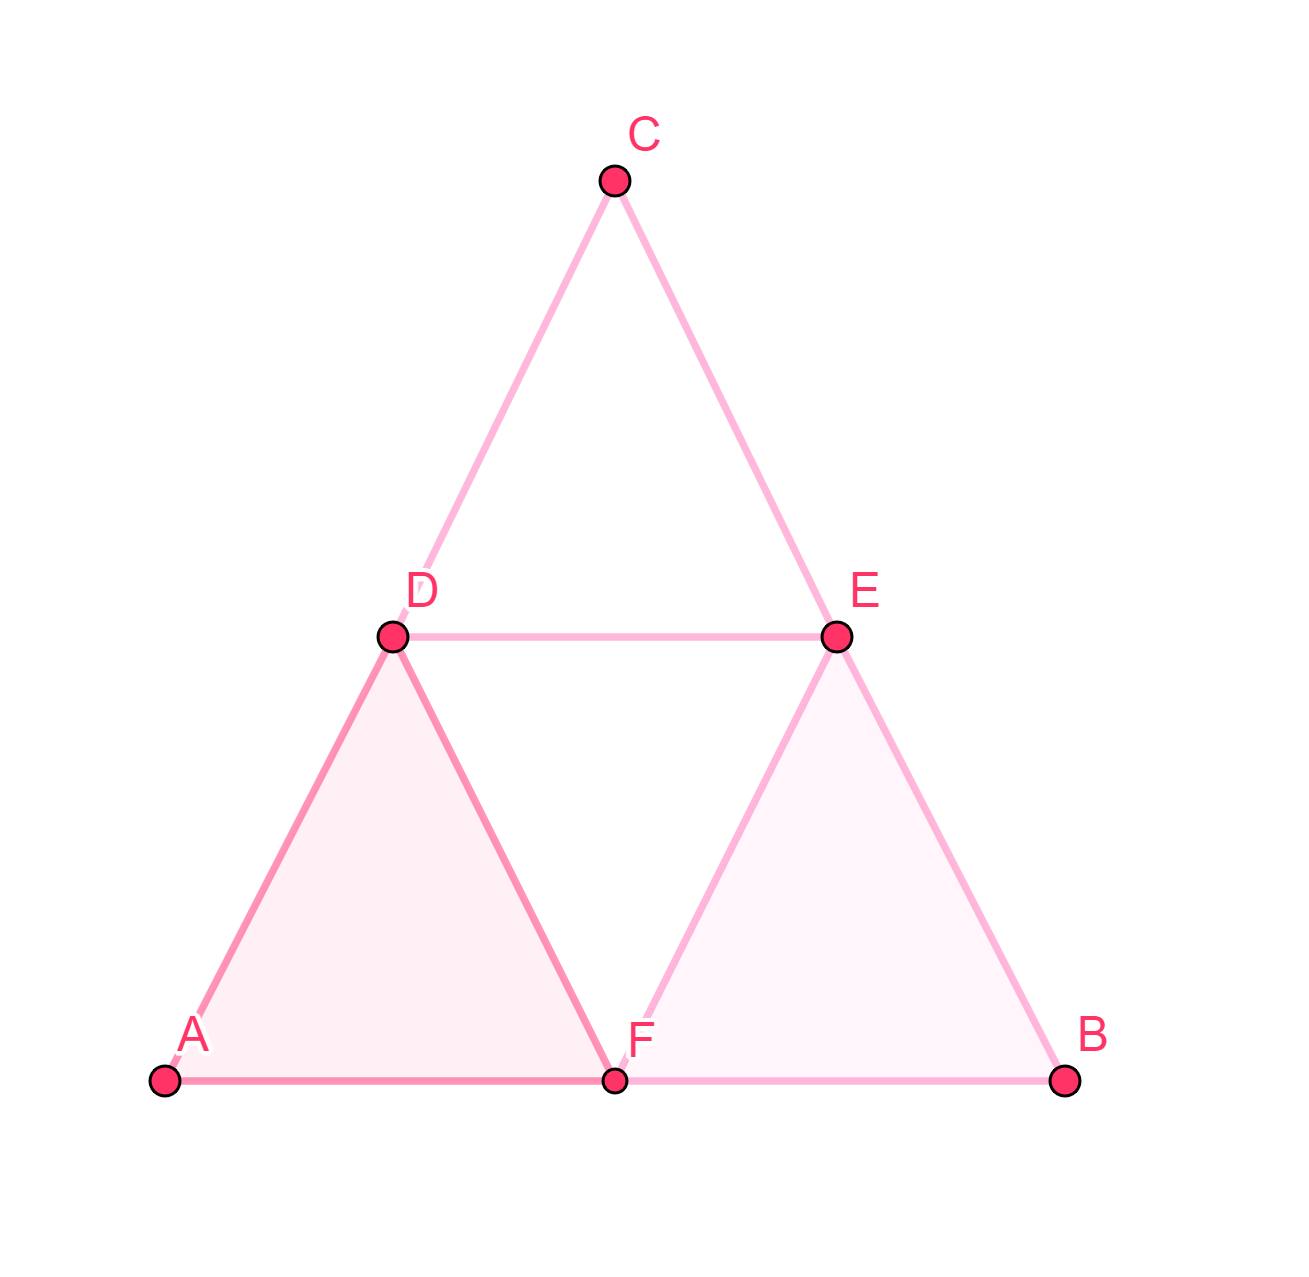
\includegraphics[scale=0.20] {graf1}
		\caption{\label{fig:1} Drawing of a simplicial complex $X$ from exercise $2$. }
	\end{figure}
	
	\textbf{(b)} $$C_2 = \langle AFD, FBE \rangle $$
	$$C_1 = \langle AF, AD, FD, FB, FE, BE, DE, DC, EC \rangle $$
	$$C_0 = \langle A, B, C, D, E, F \rangle $$	
	
	
	\textbf{(c)}
	The boundary homomorphisms connect the chain groups into a sequence: 
	$$\langle 0 \rangle \xrightarrow{\text{$\delta_3$}} C_2 \xrightarrow{\text{$\delta_2$}} C_1 \xrightarrow{\text{$\delta_1$}} C_0  \xrightarrow{\text{$\delta_0$}} \langle 0 \rangle$$
	
	We have 
	
	$$\delta_2(AFD) = AF + FD - AD$$
	$$\delta_2(FBE) = FB + BE - FE$$
	
	$$\delta_1(AF) = F-A$$
	$$\delta_1(AD) = D-A$$
	$$\delta_1(FD) = D-F$$
	$$\delta_1(FB) = B-F$$
	$$\delta_1(FE) = E-F$$
	$$\delta_1(BE) = E-B$$
	$$\delta_1(DE) = E-D$$
	$$\delta_1(DC) = C-D$$
	$$\delta_1(EC) = C-E$$
	
	$$\delta_0(A) = 0$$
	$$\delta_0(B) = 0$$
	$$\delta_0(C) = 0$$
	$$\delta_0(D) = 0$$
	$$\delta_0(E) = 0$$
	$$\delta_0(F) = 0$$
	
		\textbf{(d)}
		There are no cycles for $n=2$ because $X$ has two 2-simplices and there needs to be at least four, to form a 2-cycle. So,
		
		$$Z_2 = \text{ker}\delta_2 = \langle 0 \rangle $$
		
		There are four linearly independent cycles for $n=1$, namely $AF + FD - AD$, $FB + BE - FE$, $DE + EC - DC$ and $FD - FE + DE$, so: 
		
		$$Z_1 = \text{ker}\delta_1 = \langle AF + FD - AD, FB + BE - FE, DE + EC - DC,
		FD - FE + DE  \rangle $$
		
		Since $\delta_0$ maps all vertices to 0, for $n=0$ I have: 
		
		$$Z_0 = \text{ker}\delta_0 = \langle A, B, C, D, E, F \rangle$$
		
		Boundaries for $n=2,1,0$ are:
		
		$$B_2 = \text{im} \delta_3 = \langle 0 \rangle$$
		
		$$B_1 = \text{im} \delta_2 = \langle AF + FD - AD, FB + BE - FE \rangle$$
		
		$$B_0 = \text{im} \delta_1 = \langle F-A,D-A,D-F,B-F,E-F,E-B,E-D,C-D \rangle $$
		
		\textbf{(e)}	
		In this part of the exercise I calculated the homology groups with $\mathbb{Z}$ coefficients $H_n(X,\mathbb{Z})=\frac{Z_n}{B_n}$ for $n=2,1,0$:
		$$H_2=\frac{Z_2}{B_2}=\frac{\langle 0 \rangle}{\langle 0 \rangle}=\langle 0 \rangle$$
		
		$$H_1=\frac{\langle AF + FD - AD, FB + BE - FE, DE + EC - DC,
			FD - FE + DE  \rangle}{\langle AF + FD - AD, FB + BE - FE \rangle} = $$
		$$  = \langle DE + EC - DC, FD - FE + DE \rangle = \mathbb{Z} \oplus \mathbb{Z}$$
		
		$$H_0=\frac{Z_0}{B_0}=\frac{\langle A, B, C, D, E, F \rangle}{\langle F-A,D-A,D-F,B-F,E-F,E-B,E-D,C-D \rangle}= \langle A \rangle = \mathbb{Z}$$	
		
		\textbf{(f)} In this part of the exercise I calculated the homology groups with $\mathbb{Z}_2$ coefficients $H_n(X,\mathbb{Z}_2)=\frac{Z_n}{B_n}$ for $n=2,1,0$. The calculation does not change much, because in $\mathbb{Z}_2$ it holds $A=-A$ and consequently $B-A=B+A$ and so on. The equality $B+A=0$ still implies $B=A$ so for $n=0$ the elements still cancel each other out. The same also holds for other $n$. So I got: 
		
		$H_n(X,\mathbb{Z}_2)=\frac{Z_n}{B_n}$ for $n=2,1,0$:
		
		$$H_2=\frac{Z_2}{B_2}=\frac{\langle 0 \rangle}{\langle 0 \rangle}=\langle 0 \rangle$$
		
		$$H_1=\frac{\langle AF + FD + AD, FB + BE + FE, DE + EC + DC,
			FD + FE + DE  \rangle}{\langle AF + FD + AD, FB + BE + FE \rangle} = $$
		$$  = \langle DE + EC + DC, FD + FE + DE \rangle = \mathbb{Z}_2 \oplus \mathbb{Z}_2$$
		
		$$H_0=\frac{Z_0}{B_0}=\frac{\langle A, B, C, D, E, F \rangle}{\langle F+A,D+A,D+F,B+F,E+F,E+B,E+D,C+D \rangle}= \langle A \rangle = \mathbb{Z}_2$$	
		
		\textbf{(g)} 
		
		The Betti numbers of $X$ are $b_2=0$, $b_1=2$ and $b_0=1$.
		
		The Euler characteristic of $X$ is $\chi(X)=1-2+0=-1$.
		
		\section{Programming problems}
	
	
	
	\bibliographystyle{unsrt}
	\bibliography{references}
	
	
	% --------------------------------------------------------------
	%     You don't have to mess with anything below this line.
	% --------------------------------------------------------------
	
	
\end{document}    
